% Chapter Template

\chapter{Résultats de reconnaissance} % Main chapter title

\label{Chapitre 4.1} % Change X to a consecutive number; for referencing this chapter elsewhere, use \ref{ChapterX}

\lhead{ \emph{}} % Change X to a consecutive number; this is for the header on each page - perhaps a shortened title

%----------------------------------------------------------------------------------------
%	SECTION 1
%----------------------------------------------------------------------------------------
\section(Test de performances du système}
Ci-dessous, nous montrons les différents résultats que nous avons obtenus avec plusieures grilles.

Rapport pour le sudoku numéro 18:
\begin{center} 
\hspace{12.45cm}
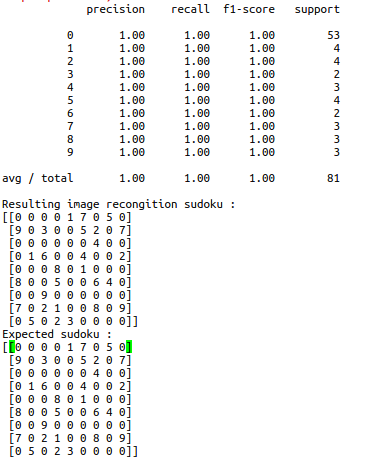
\includegraphics[width=10cm]{sudoku18.png}
\end{center}
\newpage
Rapport pour le sudoku numéro 19:
\begin{center} 
\hspace{12.45cm}
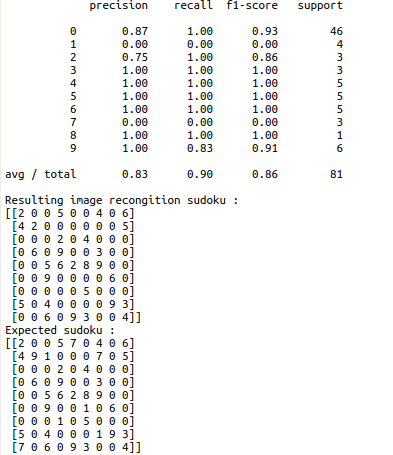
\includegraphics[width=10cm]{sudoku19.png}
\end{center}
\newpage
Rapport pour le sudoku numéro 2:
\begin{center} 
\hspace{12.45cm}
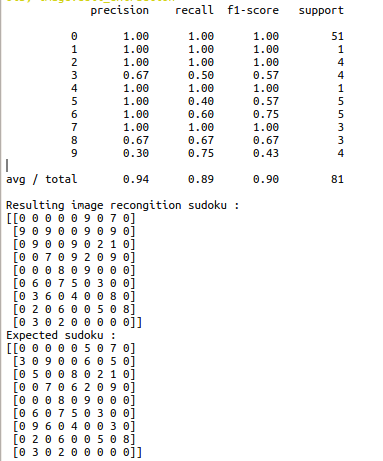
\includegraphics[width=10cm]{sudoku2.png}
\end{center}
\newpage
Rapport pour le sudoku numéro 3:
\begin{center} 
\hspace{12.45cm}
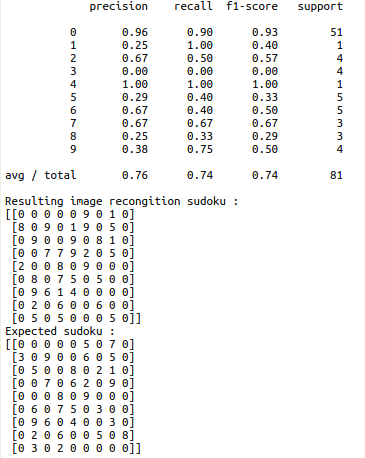
\includegraphics[width=10cm]{sudoku3.png}
\end{center}

Après étude des différents rapports pour les grilles de sudoku, nous pouvons conclure qu'avec un score de 81\%, le résultat est bon.


 


